\section{Zmniejszenie korelacji w sekwencji liczb losowych}
	\begin{frame}{Zmniejszenie korelacji w sekwencji liczb losowych}
	- procedura '' {\it losowego tasowania}'' (randoming shuffling procedure) {\it Bays, Durham 	$\Rightarrow Knuth$: ``The Art of Computer 	Programing'' vol. II.} 
	\newline \newline
	Uogólnienie:

	- kilka generatorów

	- jeden z nich wybiera ``dostarczyciela'' liczb

	\textbf{RANF} - generator systemowy,

	\textbf{RANO} - generator ulepszony

	\textbf{A} - tablica pomocnicza ( MX=97- l. pierwsza)

	\end{frame}
    
	\begin{frame}{Zmniejszenie korelacji w sekwencji liczb losowych}
		\centering 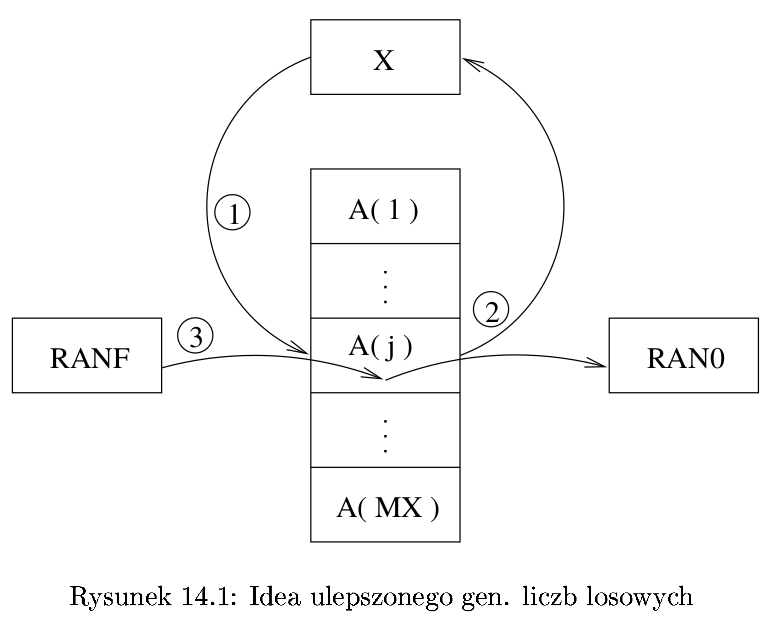
\includegraphics[width=.8\linewidth]{img/14/14_5_1_img.png}
	\end{frame}

	\begin{frame}{Zmniejszenie korelacji w sekwencji liczb losowych}
		\begin{enumerate}
			\setcounter{enumi}{-1}
			\item wypełnienie tablicy $A$ i zmiennej $x$ liczbami losowymi
			\item $x$ $\rightarrow$ $j$
			\item $A(j)$ $\rightarrow$ $l$. losowa $\rightarrow$ $x_{i}$ wyjście procedury
			\item z generatora systemowego $\rightarrow$ liczba losowa do $A(j)$
		\end{enumerate}
	\end{frame}

	\subsection{Ulepszony generator liczb losowych}
	\lstnewenvironment{code}{}{}
	
	\begin{code}
	function ran0(idum)
	parametr (MX = 97)
	real A(MX)
	data iff /0/
	
	                                     inicjacja
	if((idum.lt.0).or.(iff.eq.0)) then     -przy 1-szym
	    iff = 1                             wywolaniu
	    iseed = abs(idum)                  -gdy idum < 0
	    idum = 1
	    do 11 j = 1, MX
	        idum = ranf(iseed)             -przebiegi
	    continue                            jalowe gen.
	    do 12 j = 1, MX                     systemowego
	        A(j) = ranf(iseed)
	    x = ranf(iseed)
	endif
	
	\end{code}

	\begin{code}
	                                    przebieg roboczy
	j = 1 + int(MX * x)    - indeks
	if((j.gt.MX).or.(j.lt.1)) error()
	x = A(j)                               -z indeksu
	ran0 = x      - liczba losowa
	A(j) = ranj(iseed)                     -uzupelnienie
	return       tablicy
	end
	\end{code}
